Comecei por substituir os valores booleanos pelos respetivos valores binários e transformar o seu tipo \textit{string} no tipo numérico inteiro.

\begin{figure}[H]
    \centering
    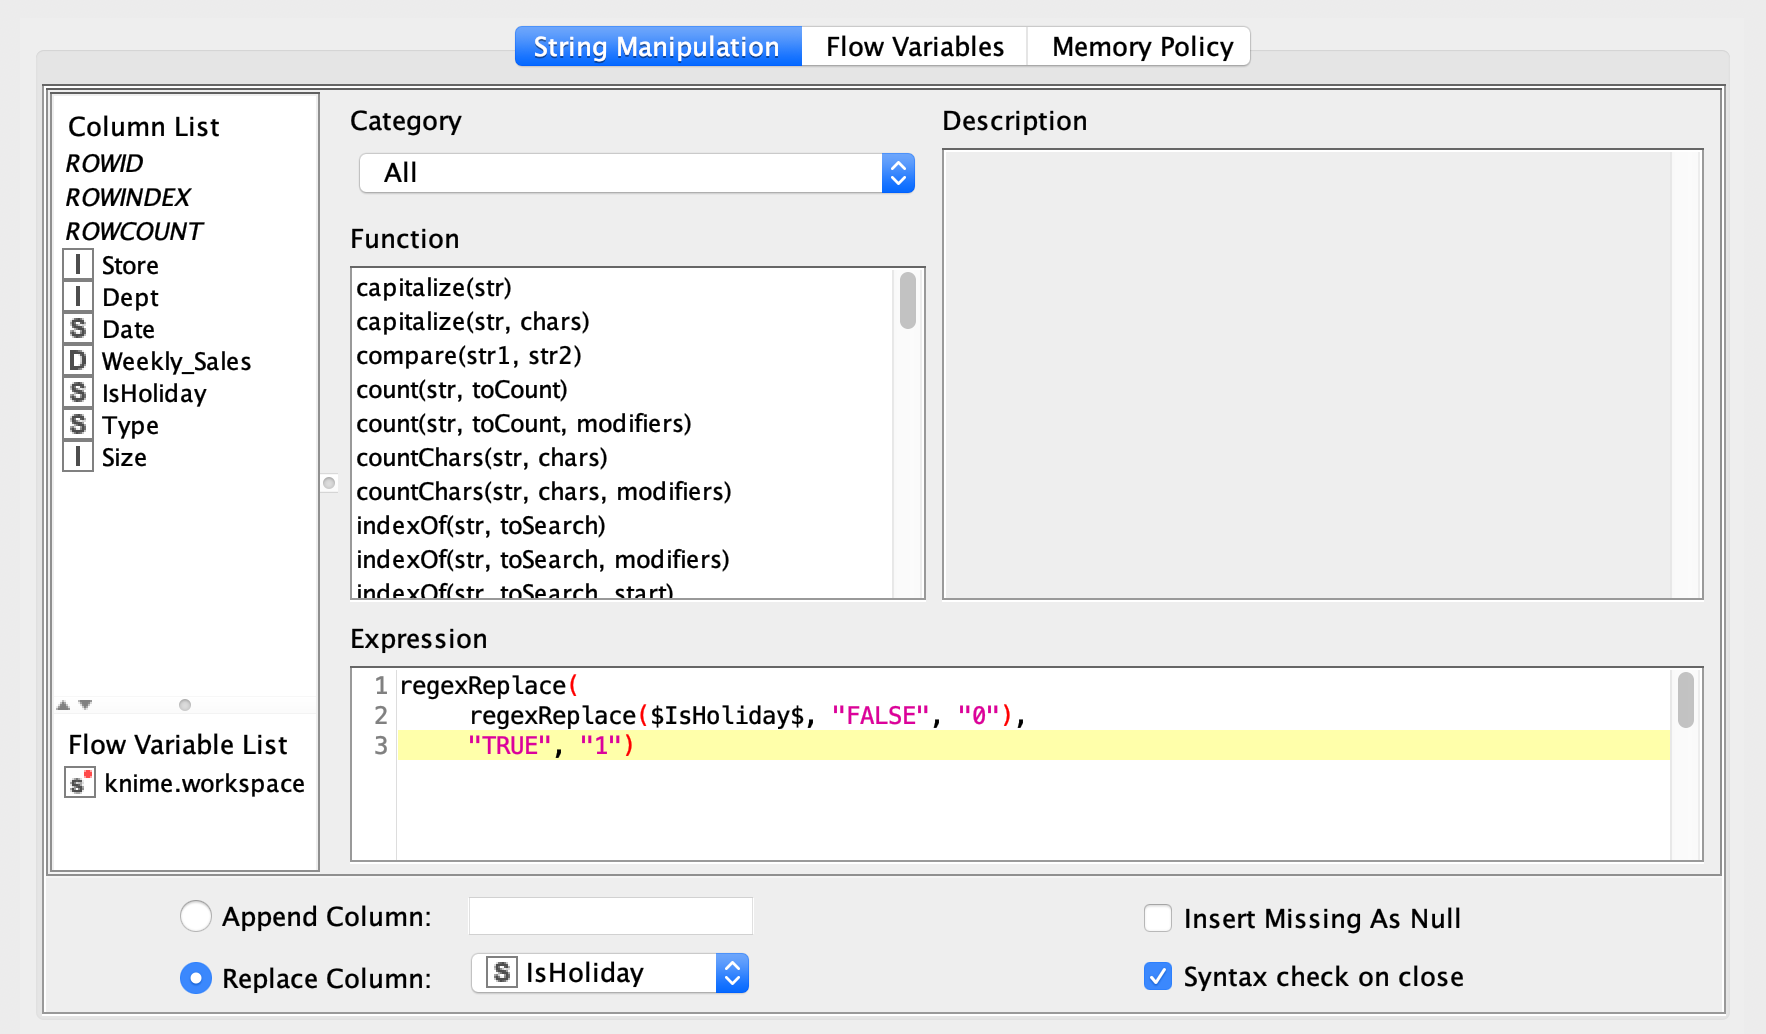
\includegraphics[scale=0.3]{Images/T2_a1.png}
    \caption{Nodo String Manipulation}
\end{figure}

\begin{figure}[H]
    \centering
    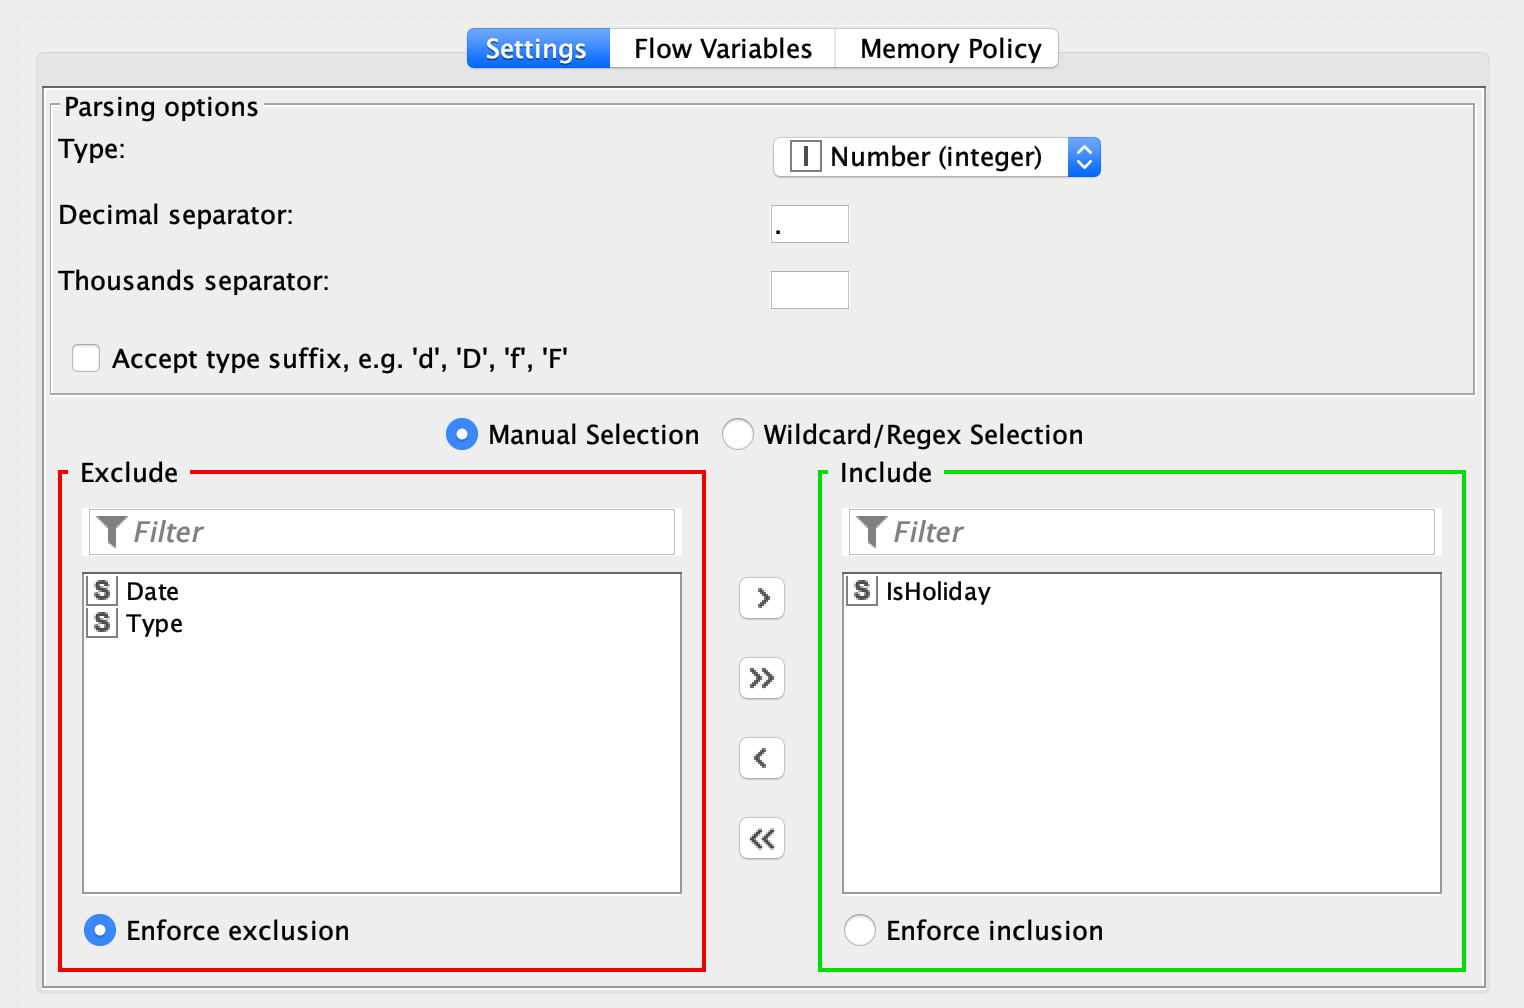
\includegraphics[scale=0.3]{Images/T2_a2.png}
    \caption{Nodo String To Number}
\end{figure}

\clearpage

Para extrair os campos ano e mês do atributo data mudei o seu tipo para \textit{Date}\&\textit{Time}. 

\begin{figure}[H]
    \centering
    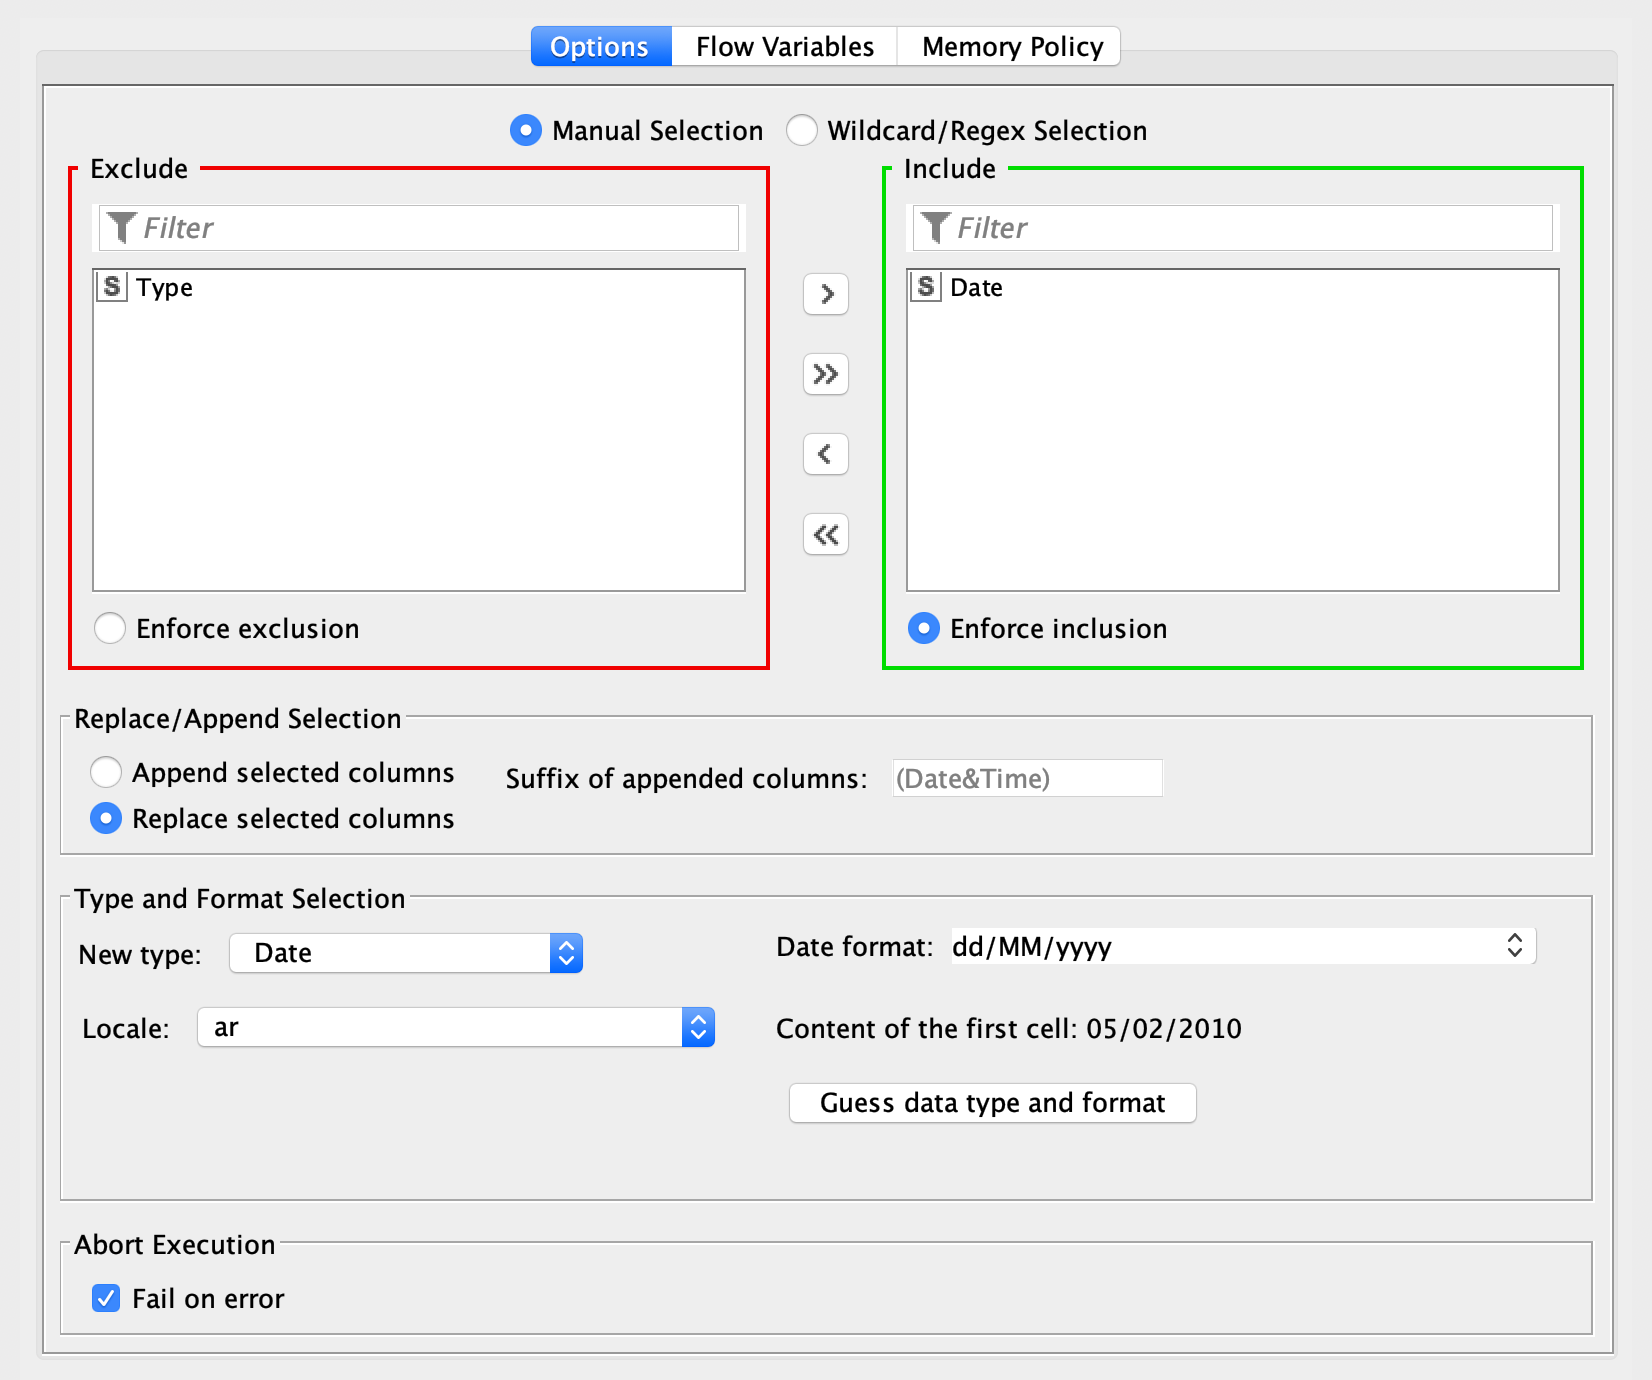
\includegraphics[scale=0.3]{Images/T2_b1.png}
    \caption{Nodo String To Date\&Time}
\end{figure}

\begin{figure}[H]
    \centering
    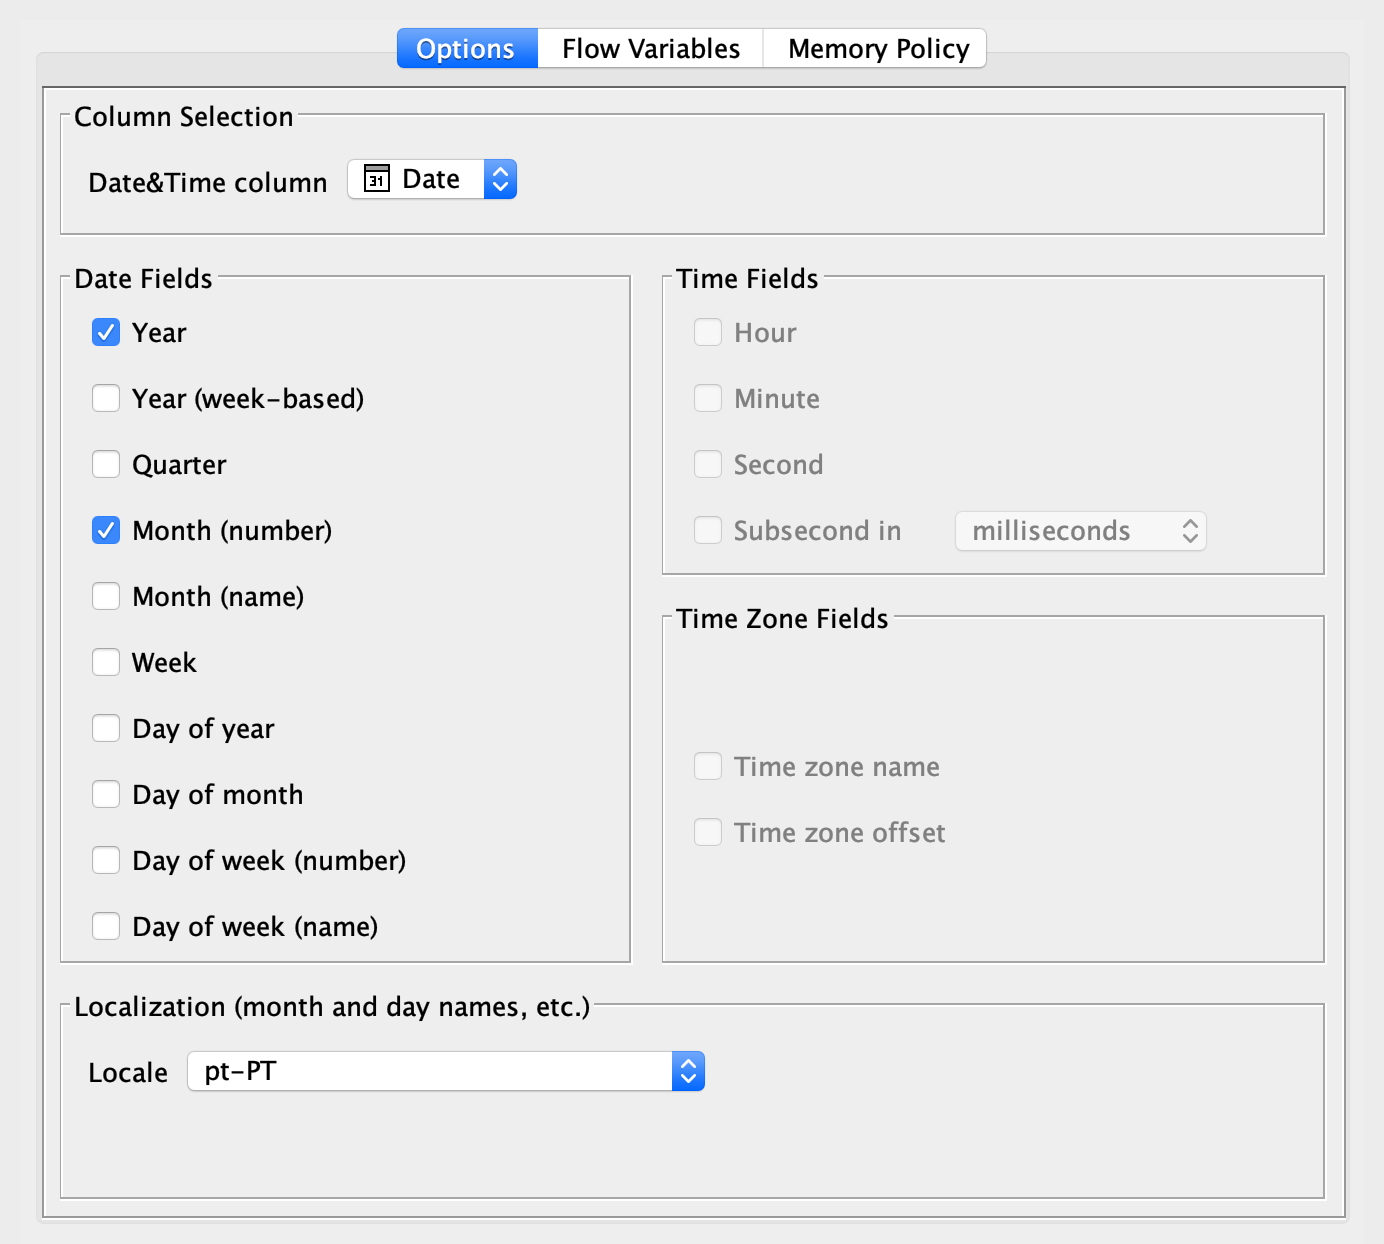
\includegraphics[scale=0.3]{Images/T2_b2.png}
    \caption{Nodo Extract Date\&Time Fields}
\end{figure}

\clearpage

Agrupando os dados pelos atributos loja, tipo, tamanho, ano e mês determinei o somatório das vendas semanais por loja, e obtendo o valor máximo do atributo \textit{IsHoliday} determinei a existência de feriados nesse mês. 

\begin{figure}[H]
    \centering
    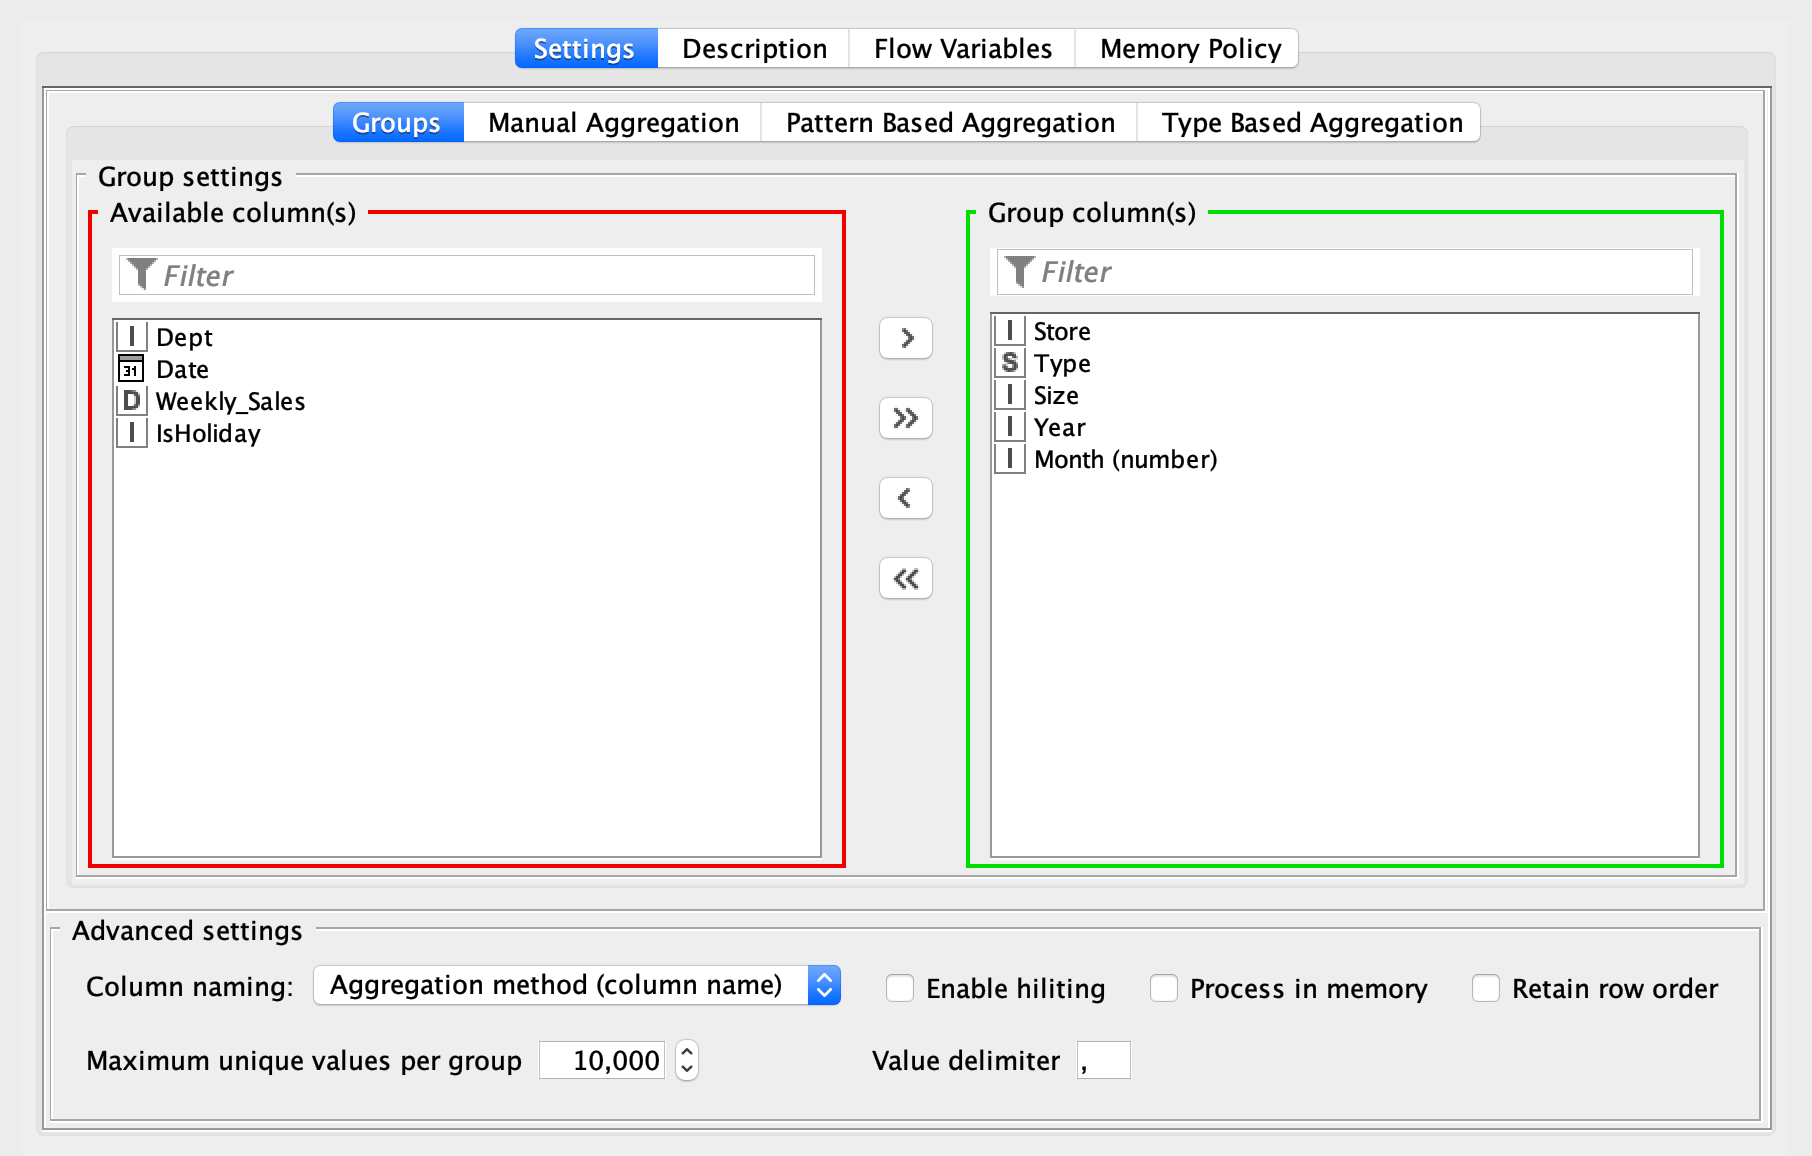
\includegraphics[scale=0.3]{Images/T2_c1.png}
    \caption{Nodo GroupBy}
\end{figure}

\begin{figure}[H]
    \centering
    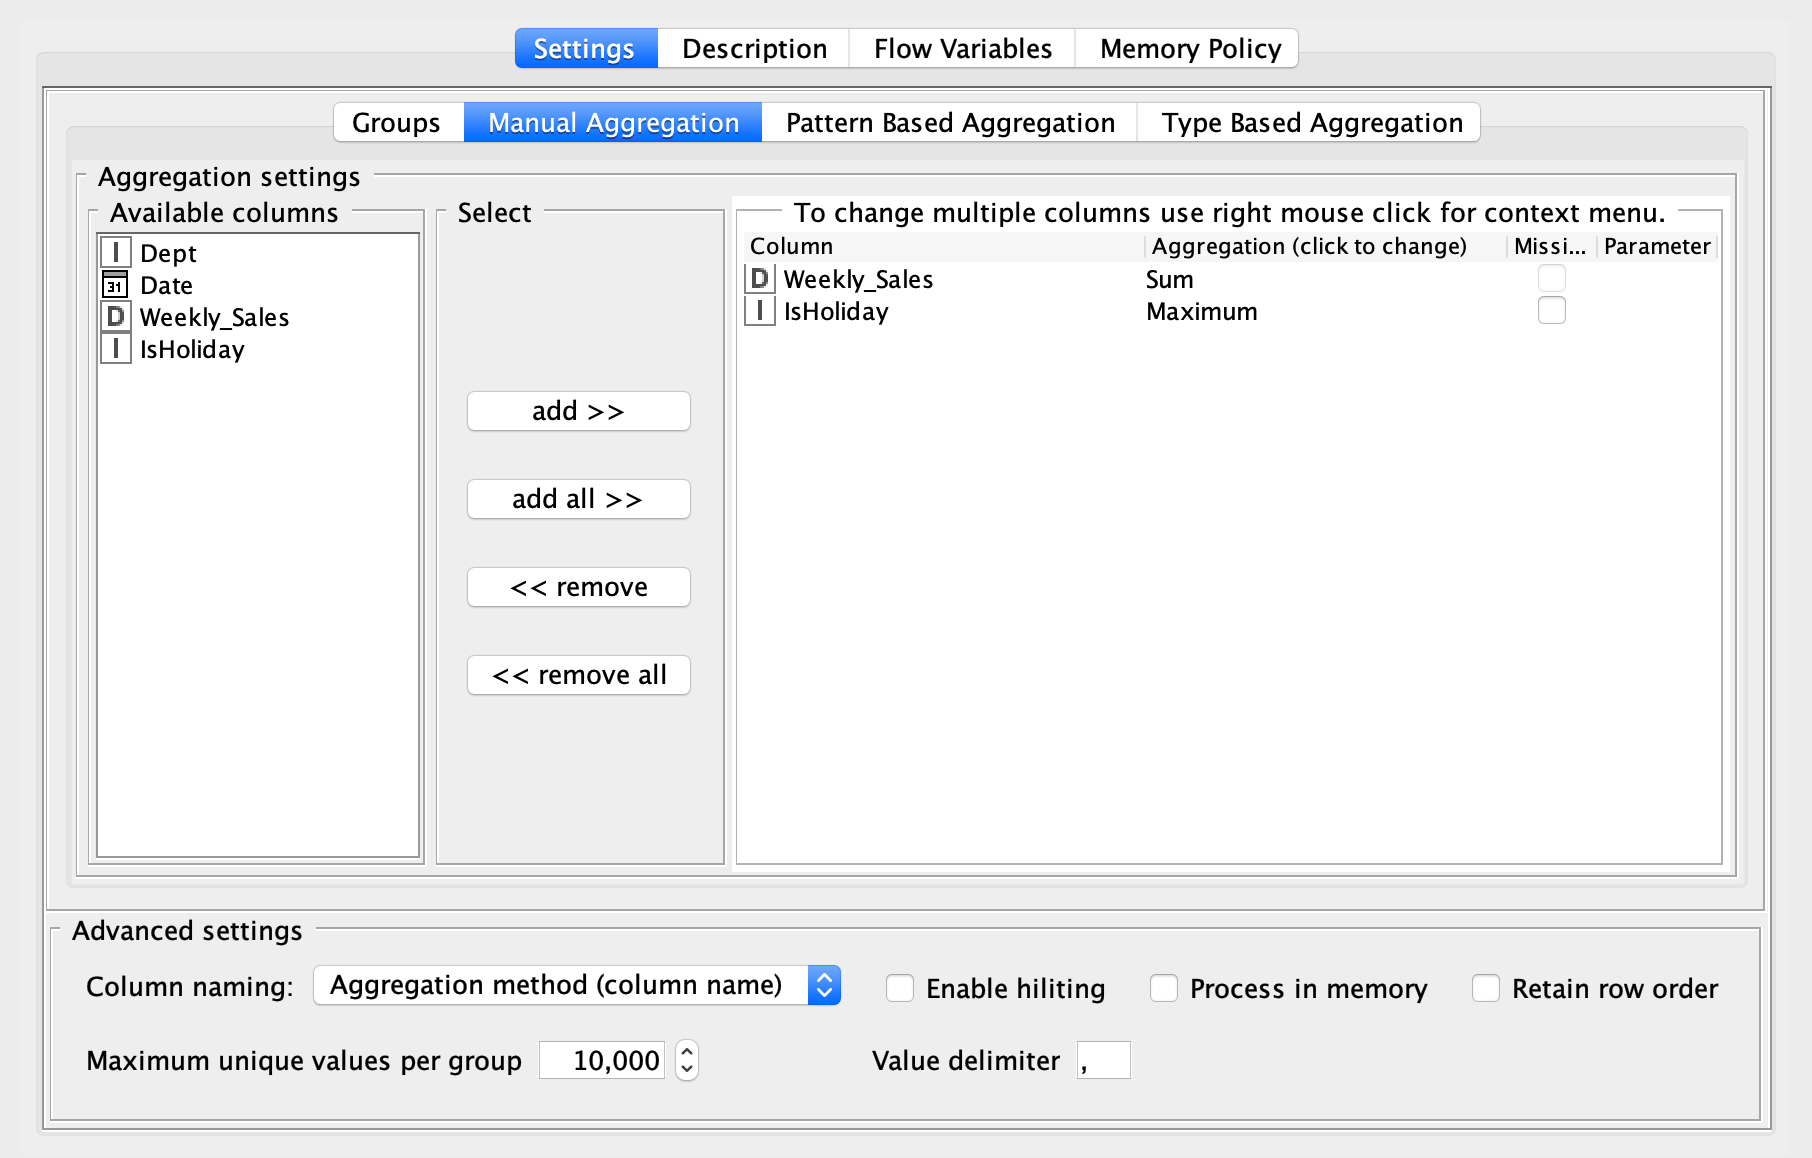
\includegraphics[scale=0.3]{Images/T2_c2.png}
    \caption{Nodo GroupBy}
\end{figure}

\clearpage

Através de uma transformação linear Min-Max entre 0 e 1 normalizei o somatório das vendas semanais.

\begin{figure}[H]
    \centering
    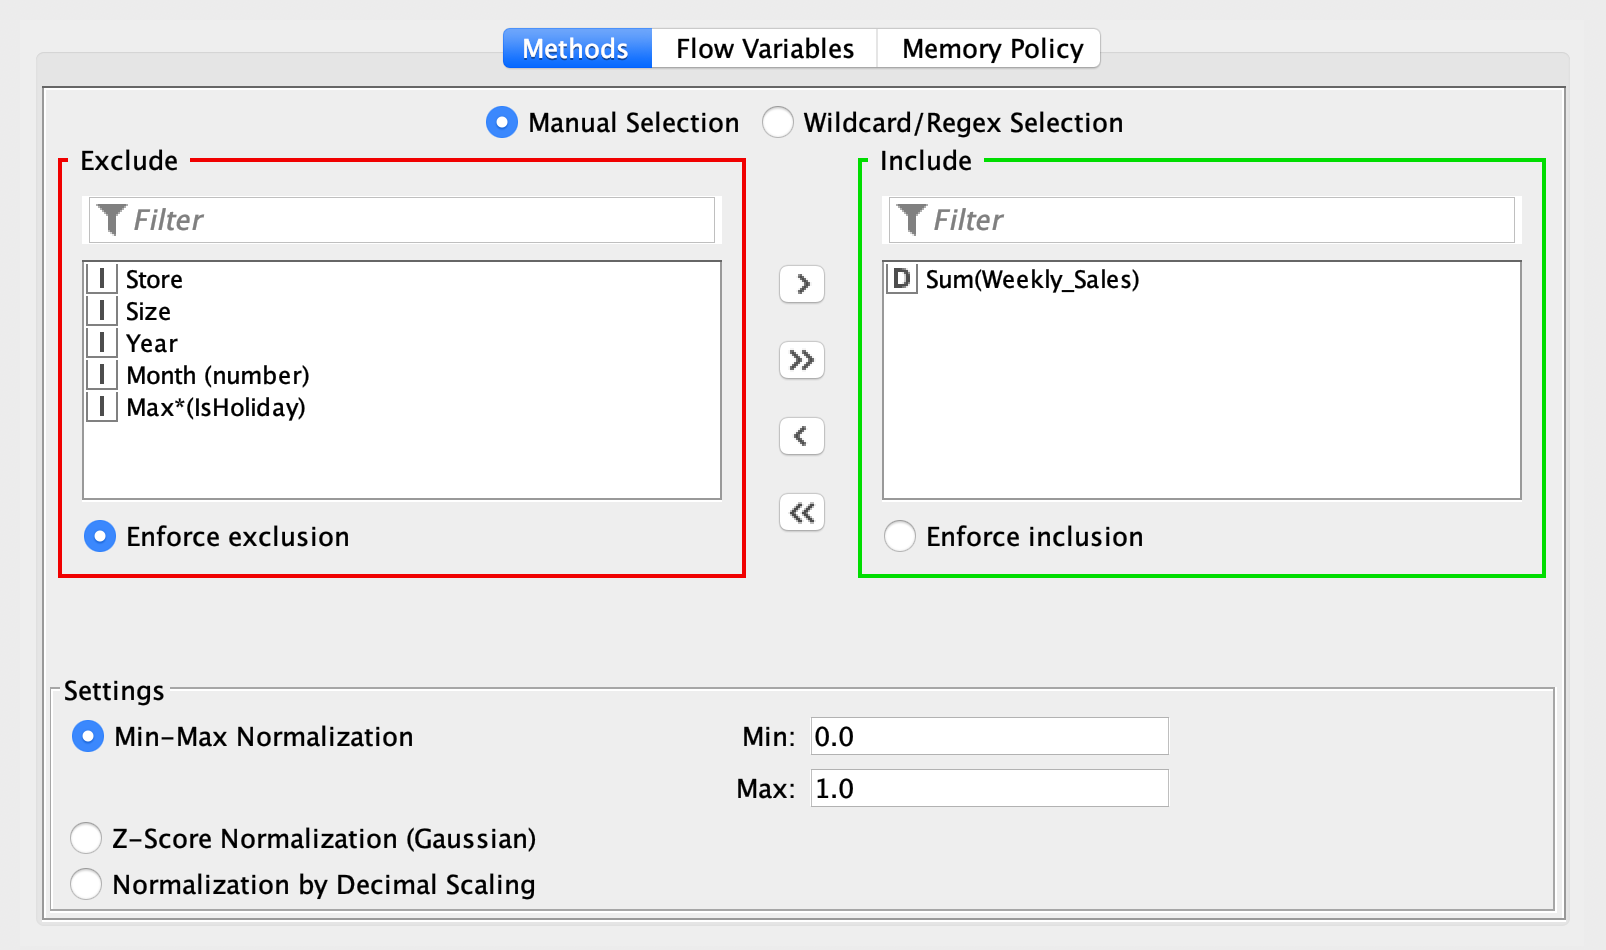
\includegraphics[scale=0.3]{Images/T2_d.png}
    \caption{Nodo Normalizer}
\end{figure}

Criei 4 bins de igual frequência sobre o valor normalizado, substituindo a respetiva coluna.

\begin{figure}[H]
    \centering
    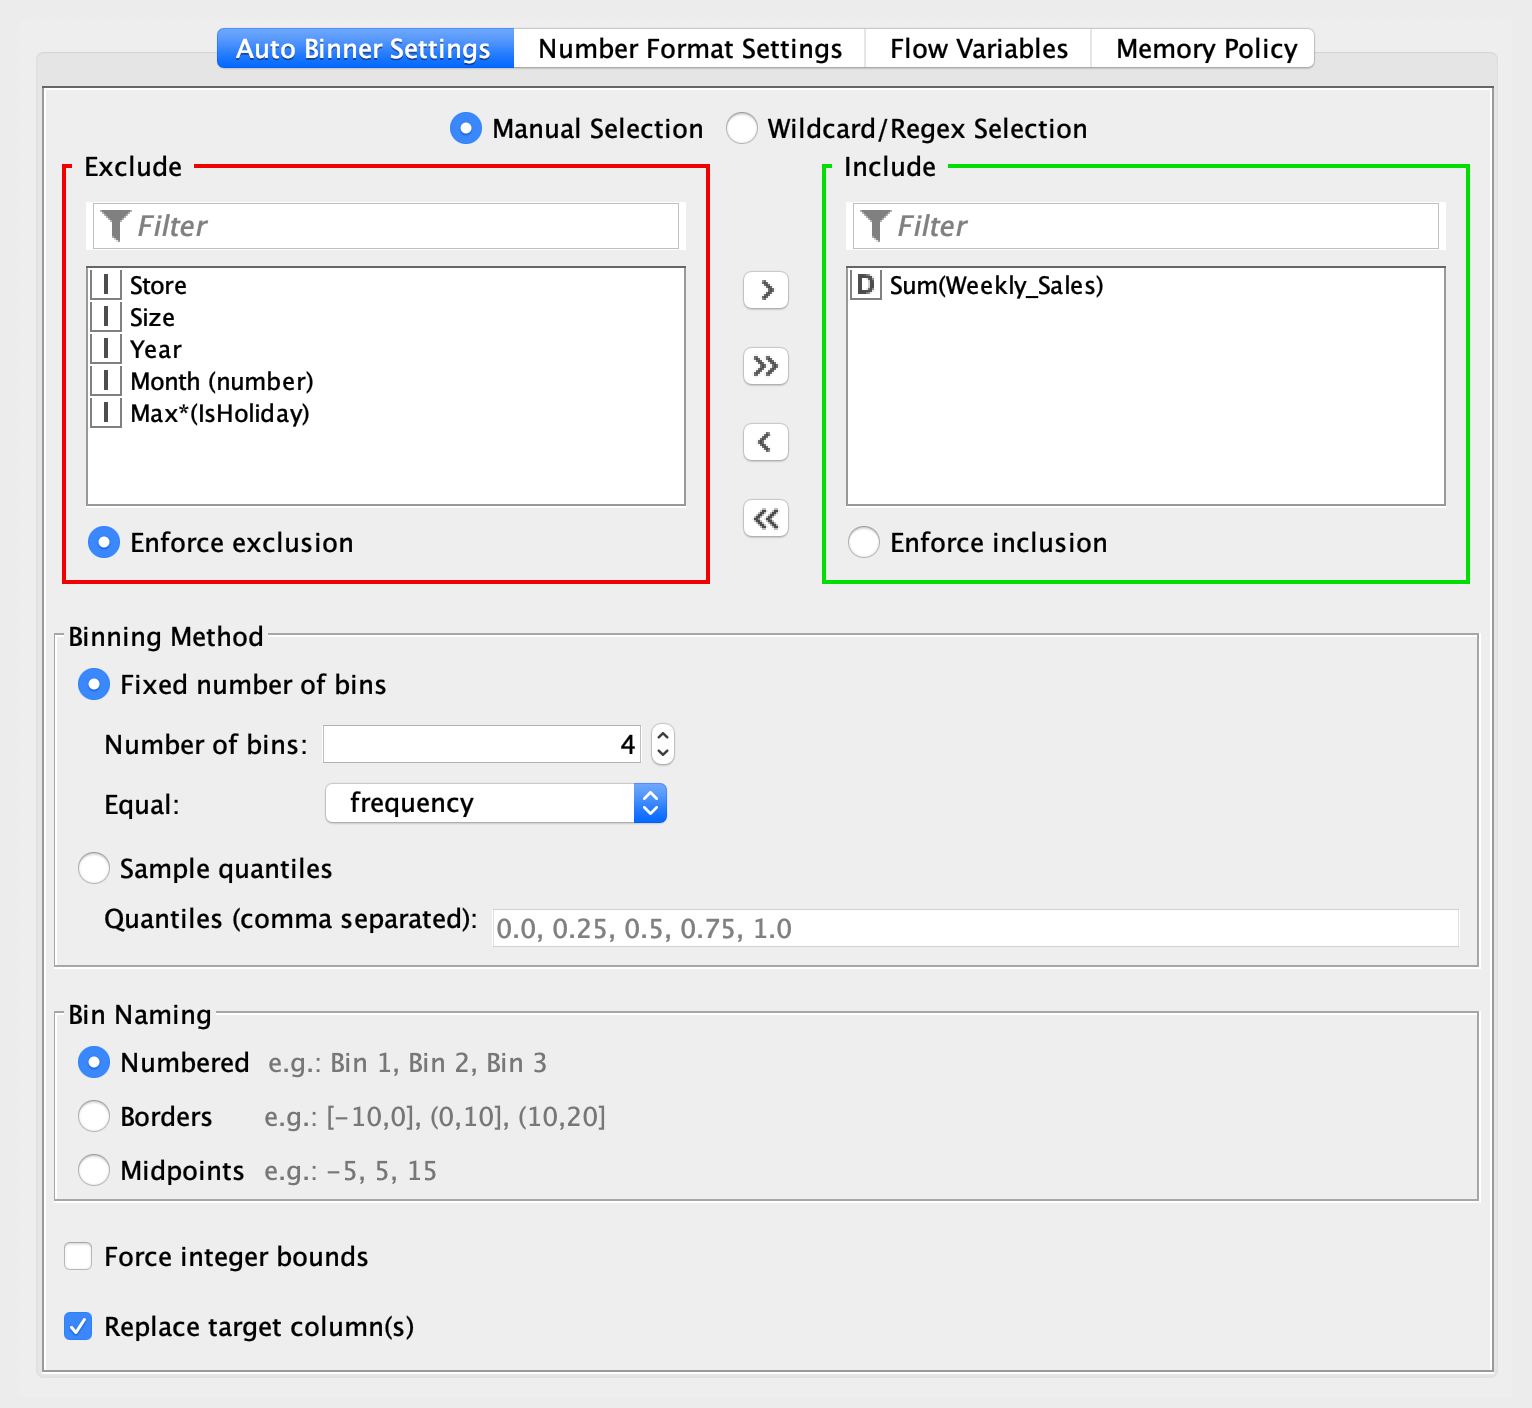
\includegraphics[scale=0.3]{Images/T2_e.png}
    \caption{Nodo Auto-Binner}
\end{figure}

\clearpage

Por fim, renomeei os bins para o respetivo valor nominal.

\begin{figure}[H]
    \centering
    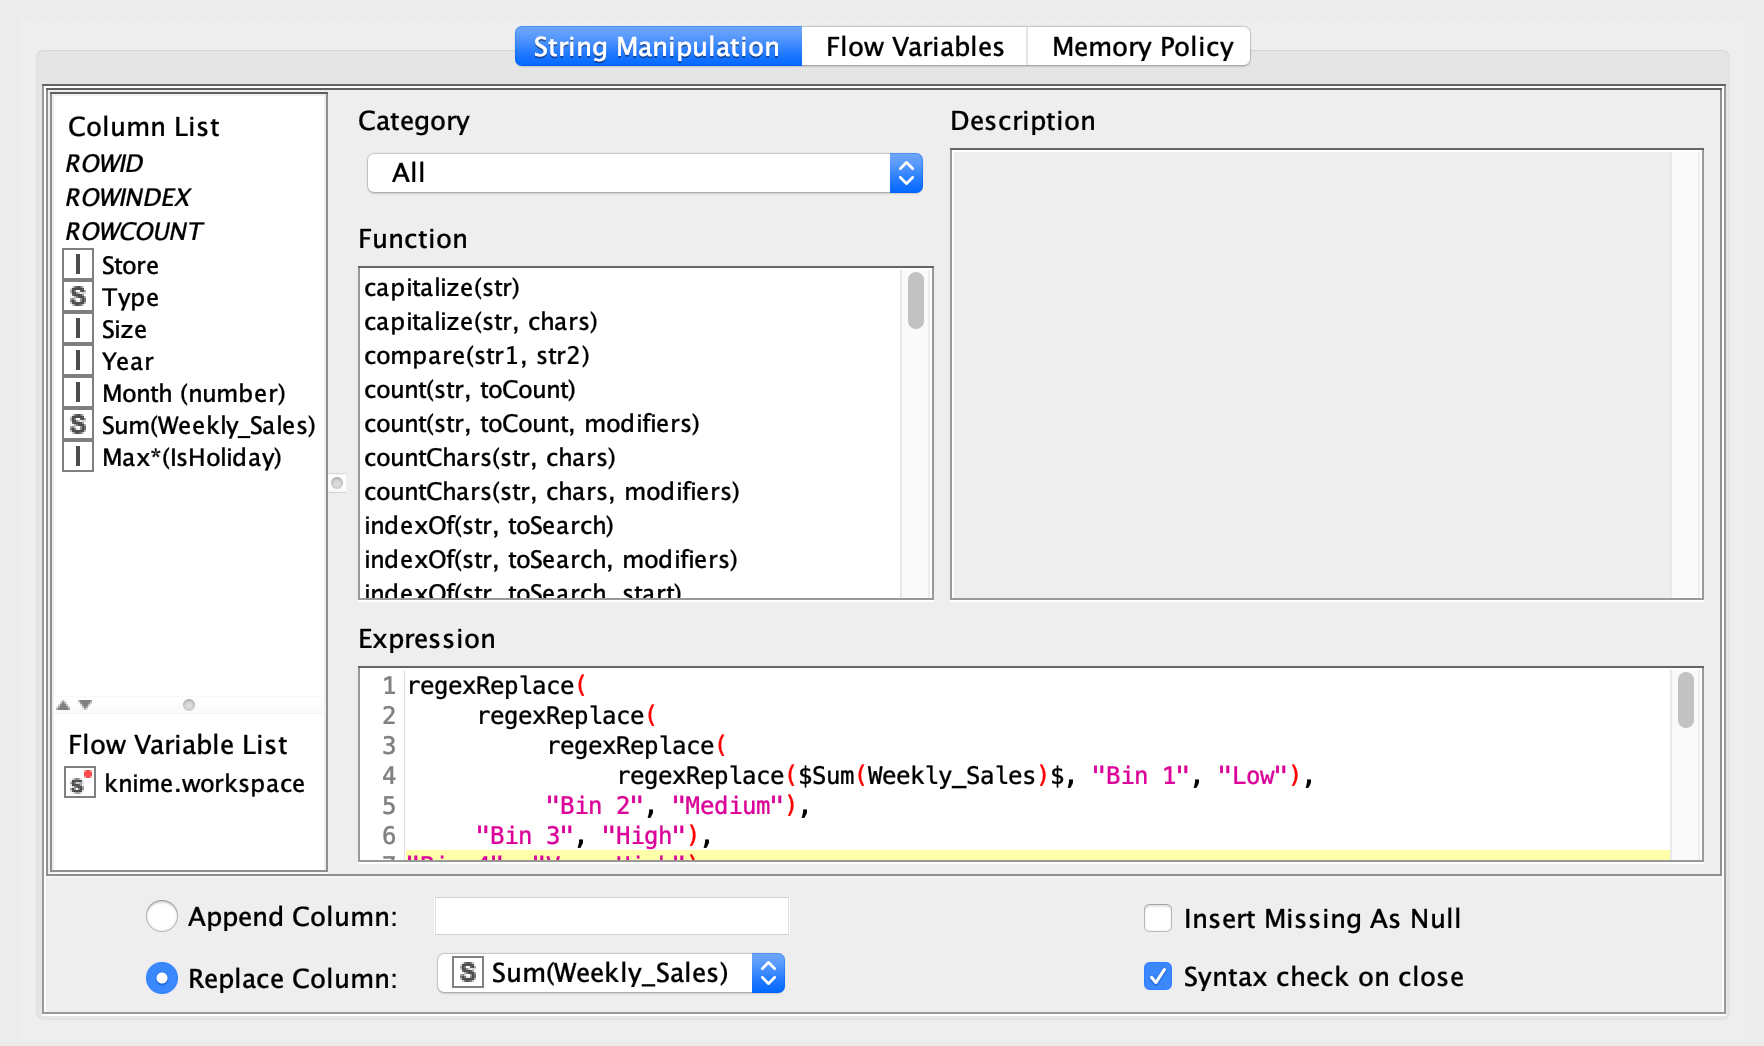
\includegraphics[scale=0.3]{Images/T2_f.png}
    \caption{Nodo String Manipulation}
\end{figure}

O seguinte workflow representa todos os passos realizados para esta tarefa.

\begin{figure}[H]
    \centering
    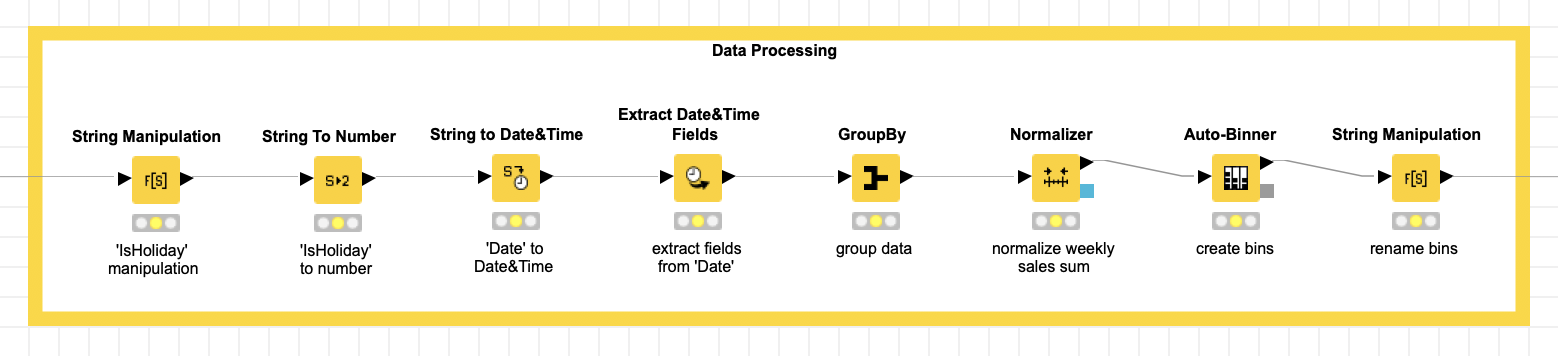
\includegraphics[scale=0.3]{Images/T2.png}
    \caption{Processamento ds dados}
\end{figure}